\documentclass{article}
% translate with >> pdflatex -shell-escape <file>

\usepackage{pgfplots}
\pgfplotsset{compat=newest}

\pagestyle{empty}

\begin{document}
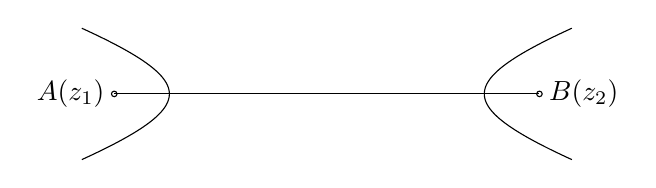
\begin{tikzpicture}%
          \draw plot[variable=\t,samples=100,domain=-50:50]
          ({2*sec(\t)},{.7*tan(\t)});
          \draw plot[variable=\t,samples=100,domain=-50:50]
          ({-2*sec(\t)},{.7*tan(\t)});
          \draw (-2.7,0) -- (2.7, 0);
          \draw (-2.7, 0) circle(1pt) (2.7, 0) circle(1pt);
          \draw (-2.7, 0) node[anchor=east] {$A(z_1)$} (2.7, 0)
          node[anchor=west] {$B(z_2)$};
\end{tikzpicture}%
\end{document}

